
\documentclass[a4paper,11pt]{article}
\usepackage[utf8]{inputenc}
\usepackage[T1]{fontenc}
\usepackage[frenchb]{babel}

\usepackage{graphicx}
\usepackage{fancyhdr}
\usepackage{geometry}

\usepackage[colorlinks,linkcolor=blue]{hyperref}
\usepackage{amsmath}
\usepackage{amssymb}
\usepackage{mathrsfs}
\usepackage{epsfig}
\usepackage {eurosym}

\usepackage{float}

\geometry{a4paper,tmargin=2cm,bmargin=2cm,lmargin=1.5cm,rmargin=1cm,headheight=2.2cm,headsep=0.5cm,footskip=1cm}
\columnsep=0.6cm

\graphicspath{{images/}} 

\usepackage{listings}
\usepackage{color}
\usepackage{xcolor}

\lstset{columns=flexible,keepspaces=true, breaklines,breakindent=0pt} 


\lstset{language=C++,
basicstyle=\ttfamily\footnotesize,
breaklines, 
keywordstyle=\bfseries\color{blue},
stringstyle=\color{red},
commentstyle=\color{blue!20!black!30!green},
morecomment=[s][\color{black}]{/**}{*/},
numbers=left,
numberstyle=\tiny\color{black},
stepnumber=2,
numbersep=10pt,
tabsize=4,
showspaces=false,
showstringspaces=false}


\fancypagestyle{plain}{
% noms des respo   dans le bas de page                                            
\lfoot{Projet de C++}
\rfoot{M.Morin J.Fourmann}
\renewcommand{\headrulewidth}{0pt}
\fancyhead{}}
% Titre a compl»ter
\title{\textbf{ \huge{Projet de programmation C++}} \\{\Large  Résolution de circuit}}

\author{
\textsc{Jérémie Fourmann} (Promo 2013 - Eléctronique - Enseeiht)\\ %mettre votre nom
\textsc{Maxime Morin} (Promo 2013 - Eléctronique - Enseeiht)\\ %mettre votre nom
%\textsc{ddd dddd} (Promo - departement - respo)     %2 nom
}

\graphicspath{{images/}}

\begin{document}

\pagestyle{plain}

\maketitle
\vspace{1cm}
\renewcommand{\contentsname}{Plan}
\tableofcontents
\vspace{2cm}



\newpage


%Objectif

\section{Objectif}
Nous devons réaliser un programme en C++ permetant de résoudre des équations différentielles du 1\ier et 2\ieme ordre à coefficients constants.
Nous allons utliser une méthode de résolution numérique de type différences finie. Nous utliserons plus particulierement la méthode d'Euler.

L'utilisateur du programme pourra via un terminal :
\begin{itemize}
 \item choisir le type de circuit (1 ou 2 ordre)
 \item choisir les valeur de ces composants
 \item choisir le type de source (c'est a dire le second membre de l'equation différentielle)\\
\end{itemize}

\paragraph{remarque : }Le pas et la durée de la simulation sont réglés par défaut. L'utilisateur n'y a pas accès. Nous n'avons pas voulu implémenter 
cette fonctionnalité pour ne pas surcharger le programme, d'autant plus qu'elle n'apporte pas plus de concept orienté objet. 


\paragraph{}Le programme ecrira dans le terminal ou dans un fichier formaté la solution numérique trouvée. 
Il sera alors possible de la tracer (voir annexe Gnuplot).\\

Nous allons à présent détailler et expliquer la structure de notre programme et les choix que nous avons a fait. Puis nous commenterons les 
résultat obtenus sur les divers circuits. 
Une fois notre code opérationel nous regarderons les limites de la éthode d'Euler.\\
En annexe nous détaillons notre méthode pour obtenir et tracer les résultats via un script élementaire unix et le programme Gnuplot.
\newpage

\section{Organistion du code}
  \subsection{Le concept général}
  Nous devons nous familiariser avec les notions de classe, héritage, polymorphysme .\\
  En effet en fonction du type de circuit la méthode de
  résolution n'est plus la meme, nous faisons donc appel a la notion de polymorphysme pour résoudre se problème. Dans notre cas les fonctions 
  circuitSolve() et diffsolve() auront plusieurs versions possible en fonction du circuit.
  \subsection{L'objet circuit}
    \begin{figure}[H]
	 \begin{center}
	  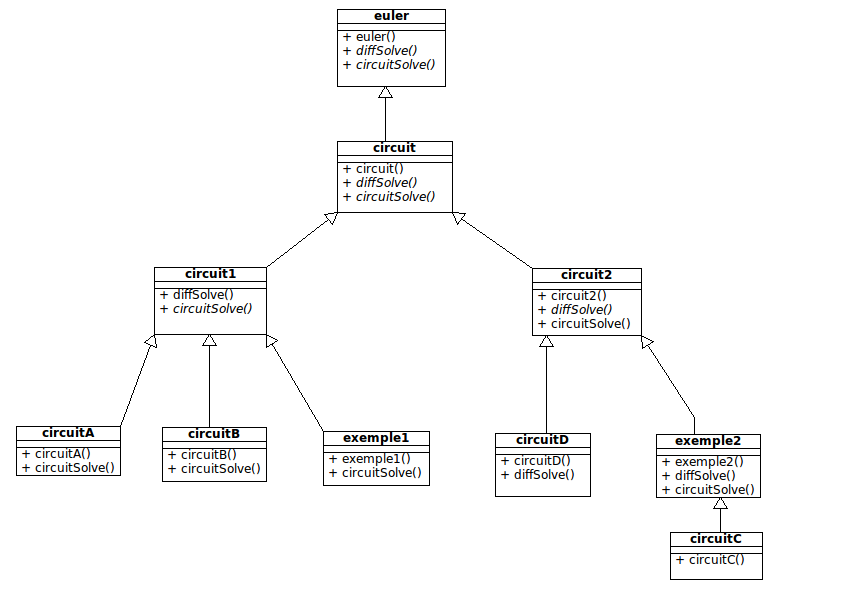
\includegraphics[scale=.5]{circuitDiagram}
	\caption{Hièrarchie de la classe circuit}
	\end{center}
      \end{figure}
    \textbf{Les principales caractéristique de cet objet :}\\

\noindent La classe Euler :
\begin{itemize}
 \item permet de définir les paramètres de simulation
  \item 2 méthode circuitSolve() et diffSolve() en virtuelles qui permettrons la résolutions du problème en fonction de la classe instancièe
\end{itemize}
La classe Circuit :
\begin{itemize}
 \item Hérite d'Euler
  \item Son constructeur permet le choix de la Source 
\end{itemize}
La classe Circuit1:
\begin{itemize}
 \item Hérite de circuit
  \item définition de la fonction circuiSolve(),qui permet de calculer résoudre au'+bu=E  
\end{itemize}
La classe Circuit1:
\begin{itemize}
 \item Hérite de circuit
  \item définition de la fonction circuiSolve(),qui permet de calculer résoudre au''+bu'+cu=E  \\
\end{itemize}

\noindent Les autres classes, héritant de ces 2 dernières, permettent de résoudre les circuit A,B,C,D, nous avons essayé de relier les exemples 
dans le cas général en considérant leurs seconds membres commes des sources particulières. \\

  \subsection{L'objet source}
    \begin{figure}[H]
	 \begin{center}
	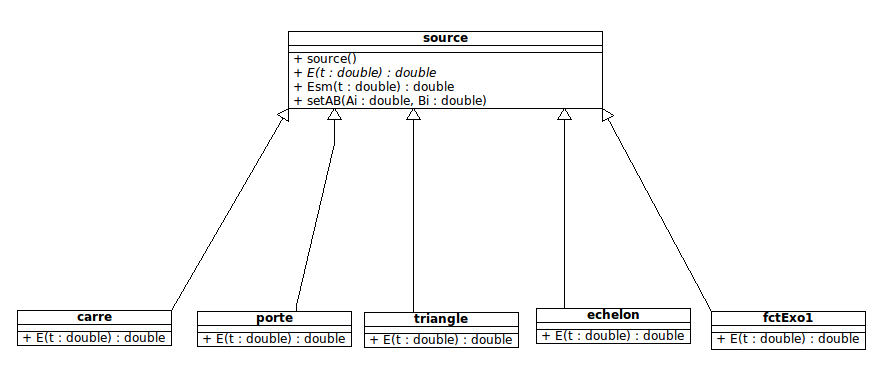
\includegraphics[scale=.5]{sourceDiagram}
	\caption{Hièrarchie de la classe source}
	\end{center}
      \end{figure}

Les classes carré, échelon... héritent de la classe mère source. Elles définissent chacune une vesion de la fontion E(t) et règle certains
attributs qui leurs sont propres comme l'amplitude, fréquences, offset ... .\\
La fonction E(t) renvoit la valeur à l'instant t de la source. L'objet Circuit va avoir comme attributs une source (ou plutôt un pointeur sur un source), 
car elle intervient dans la définition de l'équation différentielle à résoudre (seconde membre).

\subsection{Le programme principal (main)}
Notre \textit{main} créer un pointeur vers un type de montage et l'initialise selon de choix de l'utilisateur.
Il execute ensuite la methode de résolution et d'affichage de la solution du circuit qui est diffsolve().

\paragraph{Remarque : }La seule sortie du programme est \textit{stdout}. Pour alléger au maximum le programme, nous n'avons pas voulu 
utiliser une sortie supplémentaire (vers un fichier via \textit{fpritf} par exemple). Lorsque nous voulons collecter les données de sortie 
du programme dans un fichier nous utilisons la synthaxe Unix : \textit{./programme > fichier.txt}

\newpage

\section{Résultats}
  \subsection{Exemple 1}
Résolution de l'équation différentielle du 1\ier ordre :
\begin{equation*}
 \left \{
  \begin{array}{c @{=} l}
    u'(t) & -3\cdot u(t)-3\cdot t
\\
   u(0) & 0
  \end{array}
\right.
\end{equation*} 

La solution exacte étant $u(t)=-1/3\cdot exp(-3t)-1/3$
  \begin{figure}[H]
	 \begin{center}
	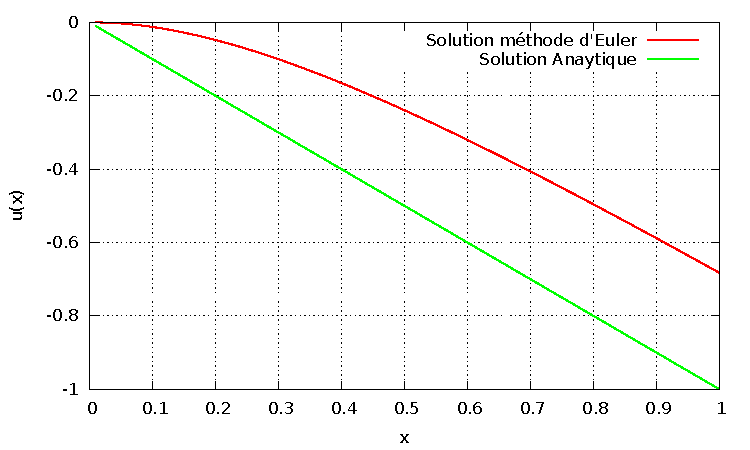
\includegraphics[scale=.8]{exemple1}
	\caption{Solution de l'exemple 1}
	\end{center}
      \end{figure}
\subsection{Exemple 2}
Résolution de l'équation différentielle du 1\ier ordre :
\begin{equation*}
 \left \{
  \begin{array}{c @{=} l}
    u''(t) & -\lambda \cdot u(t) 
\\
   u(0) & 0
\\
  u'(0)&1
  \end{array}
\right.
\end{equation*} 

La solution exacte étant $u(t)=sin(t)$

  \begin{figure}[H]
	 \begin{center}
	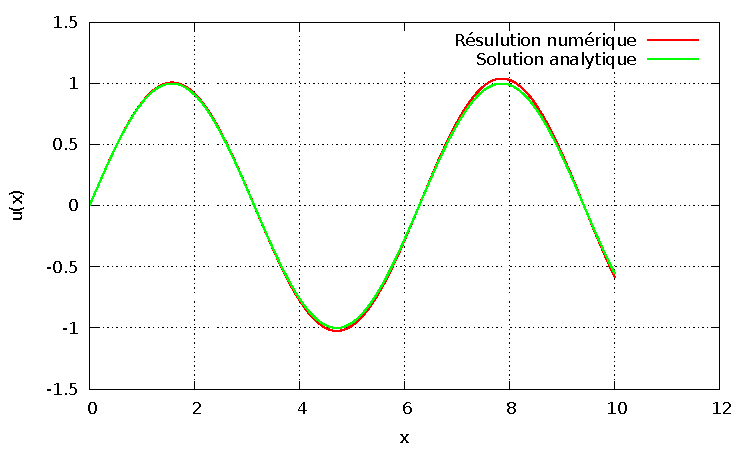
\includegraphics[scale=1]{exemple2}
	\caption{Solution de l'exemple 2}
	\end{center}
      \end{figure}

\newpage


  \subsection{Réponse du CircuitA}
  \begin{figure}[H]
	 \begin{center}
	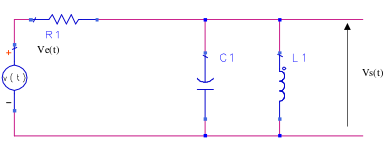
\includegraphics[scale=.7]{circuitTest}
	\caption{Circuit A}
	\end{center}
      \end{figure}
   Le circuit A est un circuit RC du 1\ier ordre, régit par l'équation différentielle :
   \begin{equation*}
    Vs+RC\cdot Vs'=Ve
   \end{equation*}
  Nous allons étudier la réponse du circuit A à plusieur type d'exitation, avec comme paramètres de simulation :  \\
  \begin{itemize}
   \item R=1 et C=1
   \item durée= ,durée= 
  \end{itemize}

\begin{figure}[h!]
   \begin{minipage}[b]{0.5\linewidth}
      \centering 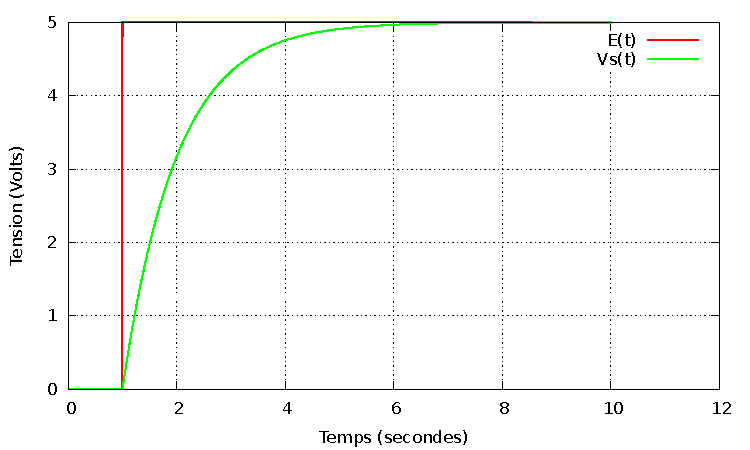
\includegraphics[scale=0.68]{CAechelon.pdf}
   \end{minipage}\hfill
   \begin{minipage}[b]{0.5\linewidth}   
      \centering 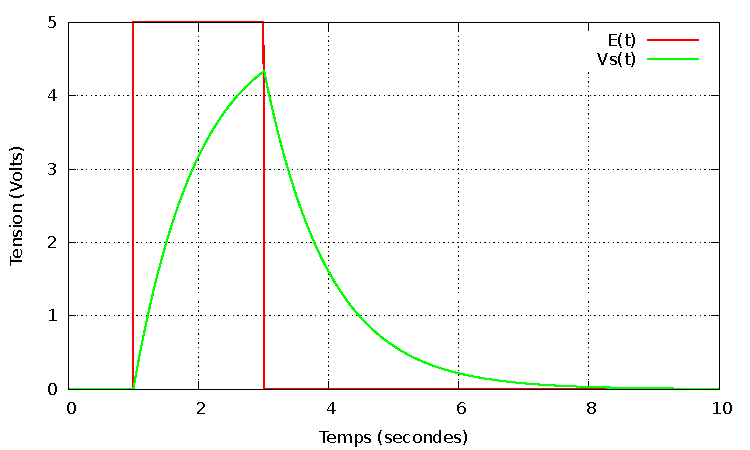
\includegraphics[scale=.68]{CAporte.pdf}
   \end{minipage}\\
    \begin{minipage}[b]{0.5\linewidth}   
      \centering 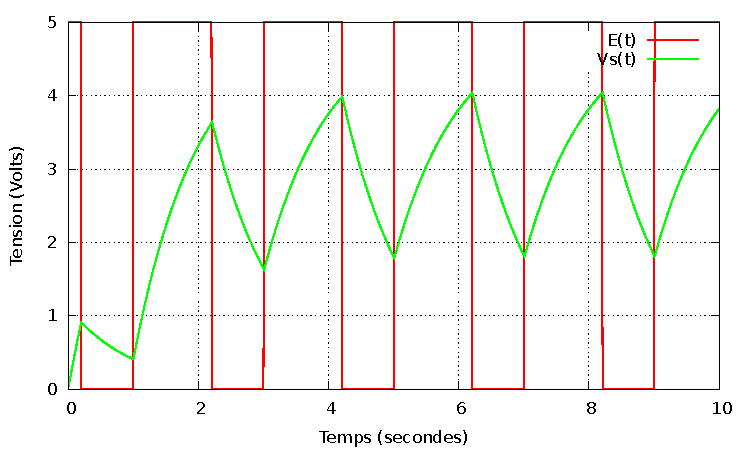
\includegraphics[scale=.68]{CAcarre.pdf}
   \end{minipage}
  \begin{minipage}[b]{0.5\linewidth}   
      \centering 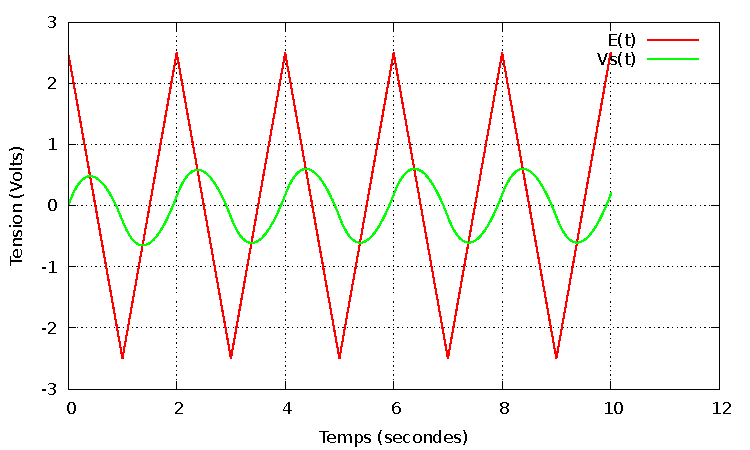
\includegraphics[scale=.68]{CAtriangle.pdf}
   \end{minipage}\\
 \caption{Réponse du circuit A}
\end{figure}

\newpage
  \subsection{Réponse du CircuitB}
  
\begin{figure}[H]
	 \begin{center}
	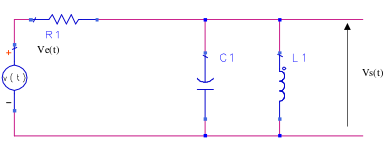
\includegraphics[scale=.7]{circuitTest}
	\caption{Circuit B}
	\end{center}
      \end{figure}
   Le circuit B est un circuit RC du 1\ier ordre, il n'est pas linéaire à cause de la diode, nous devons donc l'étudier dans 2 cas .\\
   \textbf{1er cas :} diode passante (Vd>0.6), on a une équation de charge de la capacitée .\\
   \textbf{2ième cas :} diode bloqué(Vd<0.6), on a une équationn de decharge de la capacité dans la résistance.\\
   Notre programme test la condition de Vd pour savoir quelle équation il doit résoudre, par ailleur ici on doit prendre en compte les conditions initialles.\\
   Car lors d'un changement d'équation, nous avons des conditions ``initialles''différentes .\\

   Nous allons étudier la réponse du circuit B à plusieur type d'exitation, avec comme paramètres de simulation :  \\
  \begin{itemize}
   \item R=1 et C=1
   \item durée= ,durée= 
  \end{itemize}
 
  \begin{figure}[h!]
   \begin{minipage}[b]{0.5\linewidth}
      \centering 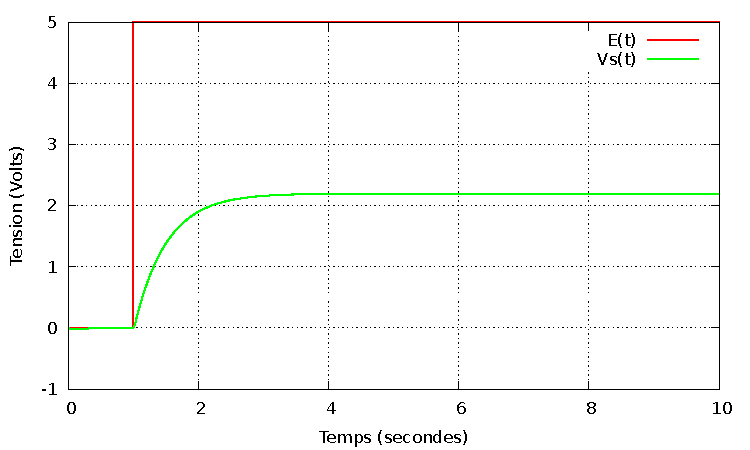
\includegraphics[scale=0.68]{CBechelon.pdf}
   \end{minipage}\hfill
   \begin{minipage}[b]{0.5\linewidth}   
      \centering 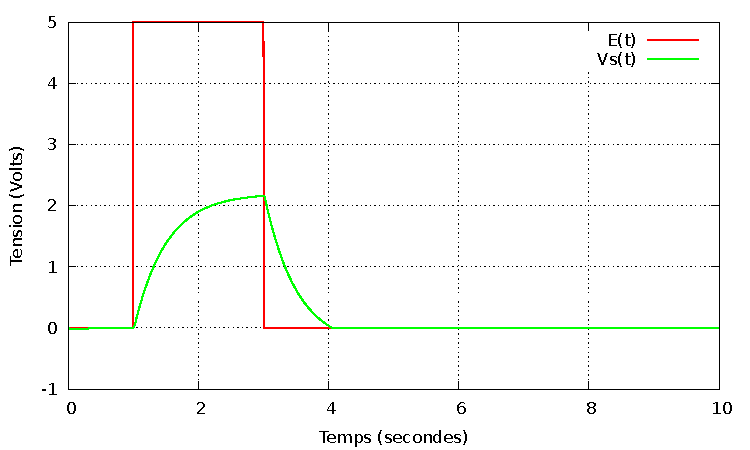
\includegraphics[scale=.68]{CBporte.pdf}
   \end{minipage}\\
    \begin{minipage}[b]{0.5\linewidth}   
      \centering 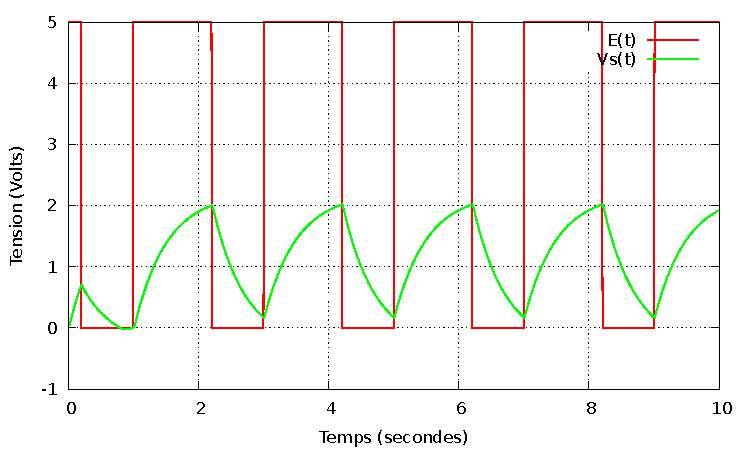
\includegraphics[scale=.68]{CBcarre.pdf}
   \end{minipage}
  \begin{minipage}[b]{0.5\linewidth}   
      \centering 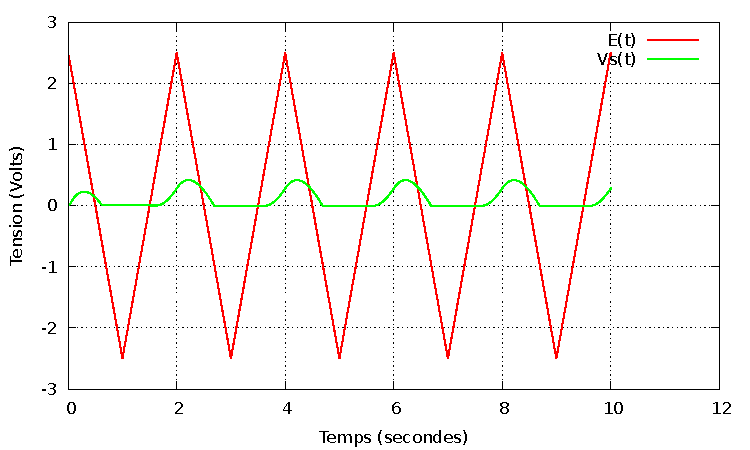
\includegraphics[scale=.68]{CBtriangle.pdf}
   \end{minipage}\\
 \caption{ Réponse du circuit B}
\end{figure}
\newpage
  \subsection{Réponse du CircuitC}

  \begin{figure}[H]
	 \begin{center}
	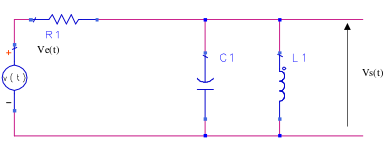
\includegraphics[scale=.7]{circuitTest}
	\caption{Circuit A}
	\end{center}
      \end{figure}
   Le circuit C est un circuit RLC du 2\ieme ordre, régit par l'équation différentielle :
   \begin{equation*}
    Todo
   \end{equation*}
  Nous allons étudier la réponse du circuit C à plusieur types d'exitations, avec comme paramètres de simulation :  \\
  \begin{itemize}
   \item R=1 et C=1
   \item pas= ,durée= 
  \end{itemize}


  \begin{figure}[h!]
   \begin{minipage}[b]{0.5\linewidth}
      \centering 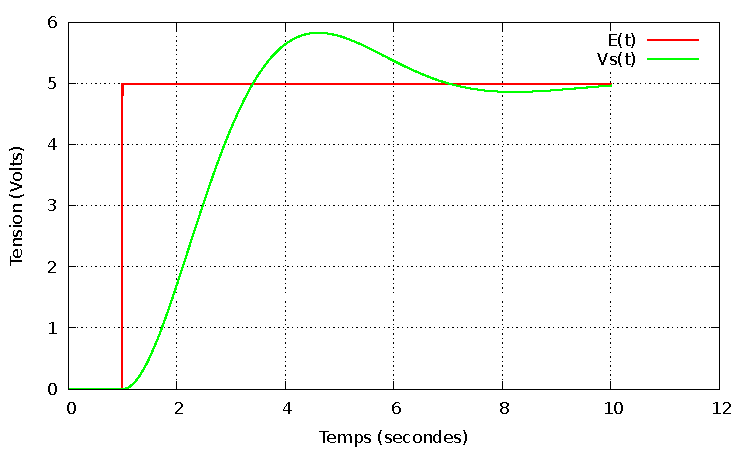
\includegraphics[scale=0.68]{CCechelon.pdf}
   \end{minipage}\hfill
   \begin{minipage}[b]{0.5\linewidth}   
      \centering 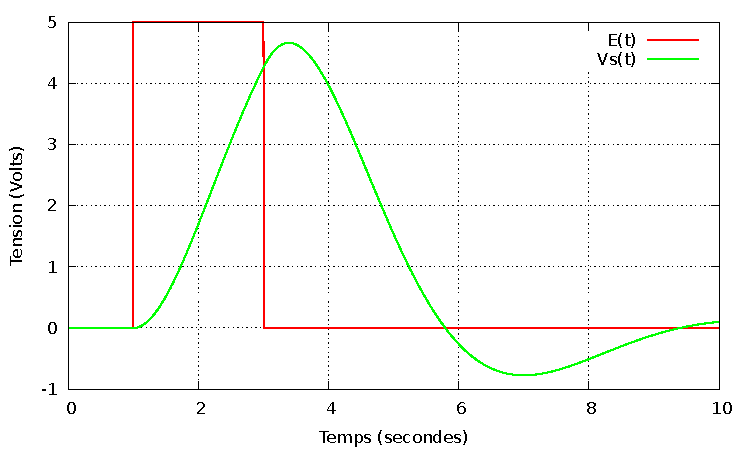
\includegraphics[scale=.68]{CCporte.pdf}
   \end{minipage}\\
    \begin{minipage}[b]{0.5\linewidth}   
      \centering 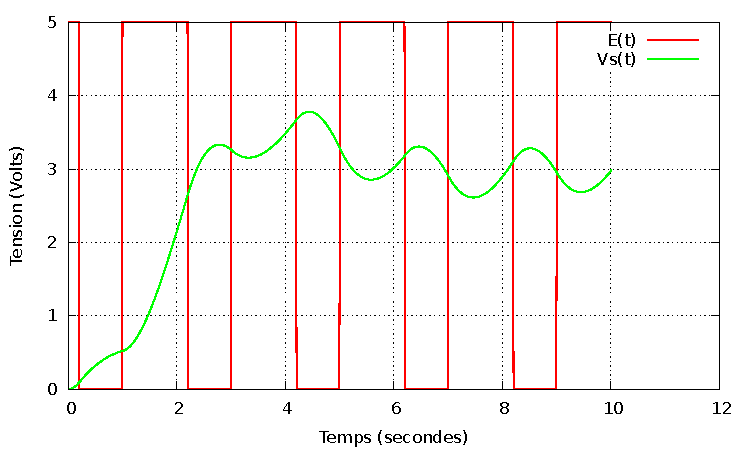
\includegraphics[scale=.68]{CCcarre.pdf}
   \end{minipage}
  \begin{minipage}[b]{0.5\linewidth}   
      \centering 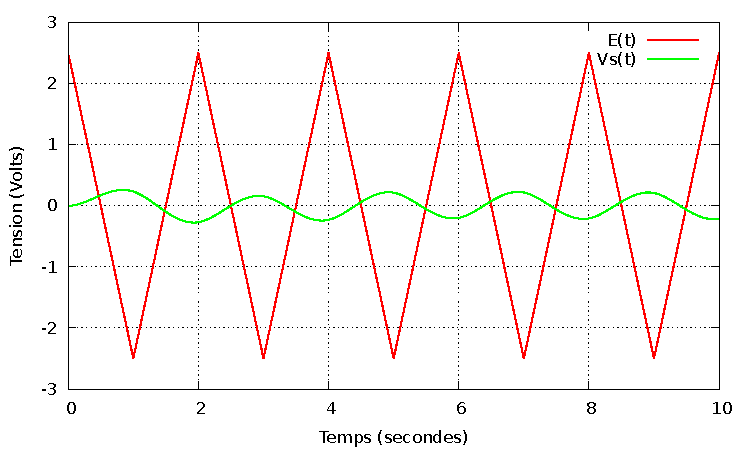
\includegraphics[scale=.68]{CCtriangle.pdf}
   \end{minipage}\\
 \caption{Réponse du circuit C}
\end{figure}

\newpage
  \subsection{Réponse du CircuitD}
  
\begin{figure}[H]
	 \begin{center}
	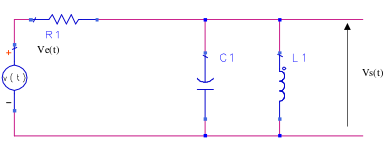
\includegraphics[scale=.7]{circuitTest}
	\caption{Circuit D}
	\end{center}
      \end{figure}
   Le circuit D est un circuit RLC du 2\ieme ordre, régit par l'équation différentielle :
   \begin{equation*}
    Todo
   \end{equation*}
  Nous allons étudier la réponse du circuit D à plusieur types d'exitations, avec comme paramètres de simulation :  \\
  \begin{itemize}
   \item R=1 et C=1
   \item pas= ,durée= 
  \end{itemize}

\begin{figure}[h!]
   \begin{minipage}[b]{0.5\linewidth}
      \centering 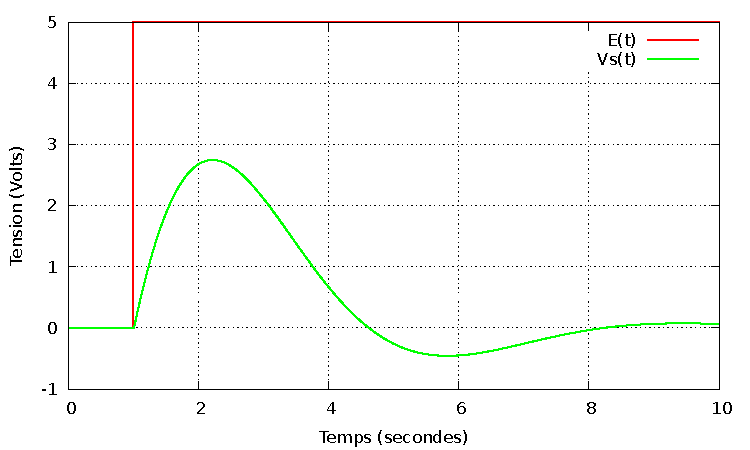
\includegraphics[scale=0.68]{CDechelon.pdf}
   \end{minipage}\hfill
   \begin{minipage}[b]{0.5\linewidth}   
      \centering 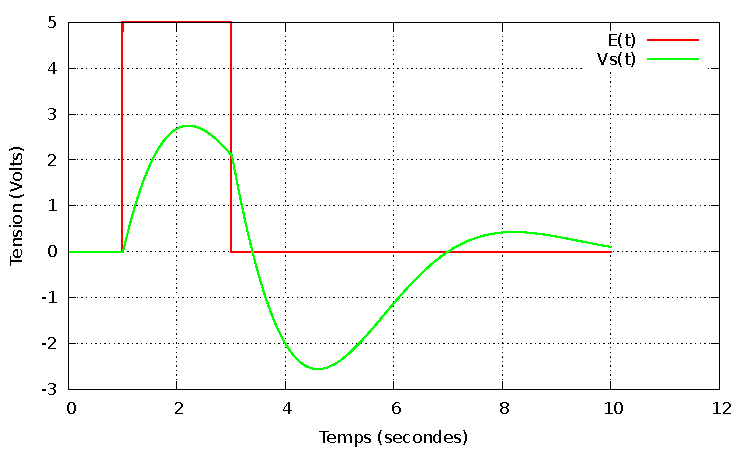
\includegraphics[scale=.68]{CDporte.pdf}
   \end{minipage}\\
    \begin{minipage}[b]{0.5\linewidth}   
      \centering 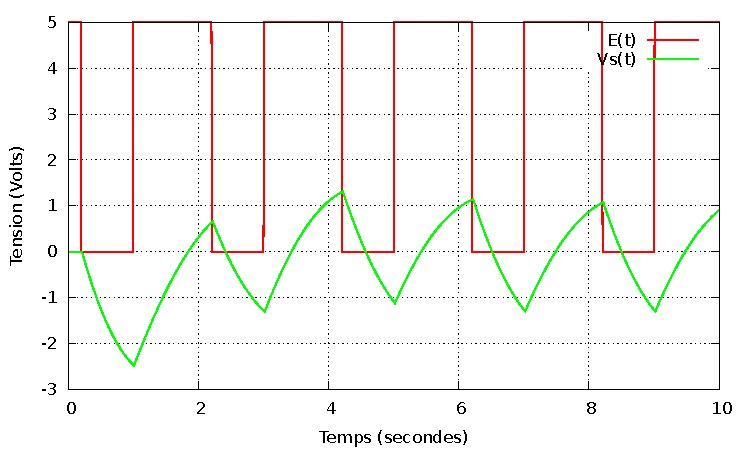
\includegraphics[scale=.68]{CDcarre.pdf}
   \end{minipage}
  \begin{minipage}[b]{0.5\linewidth}   
      \centering 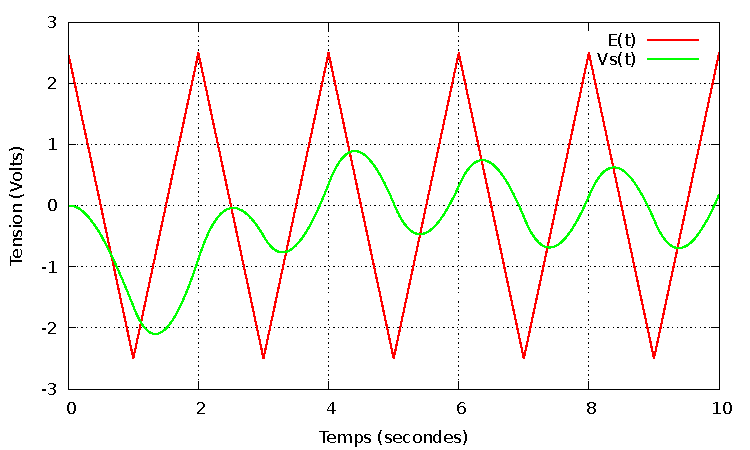
\includegraphics[scale=.68]{CDtriangle.pdf}
   \end{minipage}\\
 \caption{Réponse du circuit D}
\end{figure}




  \newpage
  \appendix
  \section{Listing du programme}
  \subsection{main.cpp}
    \lstinputlisting{../main.cpp}
    \newpage
  \subsection{circuits.h}
    \lstinputlisting{../circuits.h}
    \newpage
  \subsection{circuits.cpp}
    \lstinputlisting{../circuits.cpp}
    \newpage
   \subsection{sources.h}
    \lstinputlisting{../sources.h}
    \newpage
   \subsection{sources.cpp}
    \lstinputlisting{../sources.cpp}
    \newpage

\lstset{language=bash,
basicstyle=\ttfamily\footnotesize,
breaklines, 
keywordstyle=\bfseries\color{blue},
stringstyle=\color{red},
commentstyle=\color{blue!20!black!30!green},
morecomment=[s][\color{black}]{/*}{*/},
numbers=left,
numberstyle=\tiny\color{black},
stepnumber=2,
numbersep=10pt,
tabsize=4,
showspaces=false,
showstringspaces=false}


  \section{Script de colelcte des données et Gnuplot}
    En fainéant et pauvres étudiant que nous sommes, nous cherchions une solution rapide, gratuite et disponible chez soi pour générer les tracés 
demandés. Notre programme prend en entrée une combinaison correspondant au choix de l'utilisateur et renvoi les données dans la sortie standart.
Par exemple pour demander au programme de nous afficher les résultats de l'exemple 1 on utilise le \textit{pipe} qui dirige la sortie d'un programme 
vers l'entrée d'un autre :

\begin{lstlisting}
 echo 1 5 | ./main
\end{lstlisting}

En se plaçant évidemment au préalable dans le répertoire contenant notre fichier objet apellé \textit{main}.\\
Pour envoyer ces résultats dans un fichier on utilise le chevron :

\begin{lstlisting}
 echo 1 5 | ./main > donnees.dat
\end{lstlisting}

Automatiser la procedure revient à exécuter cette inscructions pour toutes les données demandées, c'est quasiment du copier-coller :

  \subsection{collecte.sh}
    \lstinputlisting{collecte.sh}

Les dernières lignes apellent GNUplot. Le fichier \textit{aTrace} dit au logiciel ou se trouvent les données, où il doit les tracées,
leur format de sortie, les légendes, etc... Lui aussi est un peu répétitif.

\lstset{language=GNUplot,
basicstyle=\ttfamily\footnotesize,
breaklines, 
keywordstyle=\bfseries\color{blue},
stringstyle=\color{red},
commentstyle=\color{blue!20!black!30!green},
morecomment=[s][\color{black}]{/*}{*/},
numbers=left,
numberstyle=\tiny\color{black},
stepnumber=2,
numbersep=10pt,
tabsize=4,
showspaces=false,
showstringspaces=false}

  \subsection{aTrace}
    \lstinputlisting{aTrace}

\end{document}
